\documentclass[conference]{IEEEtran}
\IEEEoverridecommandlockouts
% The preceding line is only needed to identify funding in the first footnote. If that is unneeded, please comment it out.
\usepackage{cite}
\usepackage{amsmath,amssymb,amsfonts}
\usepackage{algorithmic}
\usepackage{graphicx}
\usepackage{textcomp}
\usepackage{xcolor}
\usepackage{url}  
\usepackage[hidelinks]{hyperref}

\def\BibTeX{{\rm B\kern-.05em{\sc i\kern-.025em b}\kern-.08em
    T\kern-.1667em\lower.7ex\hbox{E}\kern-.125emX}}
\begin{document}

\title{RISC-V: ASIC-Design Team}

\author{\IEEEauthorblockN{Charlie Liu}
\IEEEauthorblockA{\textit{Electrical and Computer Engineering} \\
\textit{Rice University}\\
Houston, United States \\
cl228@rice.edu}
\and
\IEEEauthorblockN{Kelly Chan}
\IEEEauthorblockA{\textit{Electrical and Computer Engineering} \\
\textit{Rice University}\\
Houston, United States \\
kc162@rice.edu}
}

\maketitle

\begin{abstract}
The reduced instruction set computer five (RISC-V) ecosystem is growing rapidly, but a gap remains in transitioning register-transfer level (RTL) designs to manufacturable chips from the previous semesters of the RISC-V Capstone. This project aims to bridge that gap by implementing a complete application-specific integrated circuit physical design flow. It will begin from a basic ELEC 527: VLSI Systems Design framework, and then define a custom process to achieve the final Graphic Data System II (GDSII) file while optimizing power, performance, and area (PPA). Our solution includes adapting previous flows to our RISC-V core using industry standard tools such as Design Compiler and Innovus to create our own automated flow, beginning with synthesizing the RTL all the way to generating a GDSII layout. By next semester, our workflow will be completed using the basic substitute file and it should be adapted to the core design. Eventually, it will be taped out into a manufacturable chip.
\end{abstract}

\begin{IEEEkeywords}
RISC-V, physical design, RTL, GDSII
\end{IEEEkeywords}

\section{Introduction}
First, it is important to understand why reduced instruction set computer five (RISC-V) is important, and how it impacts the engineering industry and markets. According to Synopsys, “RISC-V is an open-source instruction set architecture used to develop custom processors for a variety of applications, from embedded designs to supercomputers.” [1] Since its inception in 2010, it has quickly and exponentially become an integral part of computing. Its skyrocketing popularity and projected market growth can be attributed to a few key features, including but not limited to: 

\begin{itemize}
    \item “Its open-standard nature, which allows collaboration and innovation across the industry.” \cite{b1}
    \item “Common ISA, which helps make software development easier since all processors could potentially use the same architecture. Designers can use the same base ISA, from simple embedded devices to the largest supercomputers, tailoring their device to the needs of the market. Compared to previous ISAs, RISC-V ISAs have unique features and can be customized based on their requirements.” \cite{b1}
    \item “Availability of smaller, energy-efficient, and modular options.” \cite{b1}
    \item “Security features, which are available through open-source reference designs, software composition analysis tools, and security extensions. In addition, its open-source nature means that the entire RISC-V architecture can be scrutinized closely in the public domain, eliminating back doors and hidden channels.” \cite{b1}
\end{itemize}

Thus, our project aims to take advantage of these features. The SwitchMCU, a capstone four semesters in the making, utilizes a custom RISC-V 32-bit core that has the ability to execute C programs, as well as allow for future custom instructions and additional peripherals. It is programmed as a general-purpose biomedical application processor, supports a 5-stage pipeline, and uses Harvard architecture. Furthermore, it contains synchronous and asynchronous First-In, First-Out (FIFO) data structures for data transmission, Universal Asynchronous Receiver-Transmitter (UART), Serial Peripheral Interface (SPI), and General-Purpose Input/Output (GPIO) peripherals. More can be found on the official GitHub website. \cite{b2}

\begin{figure}[htbp]
    \centering
    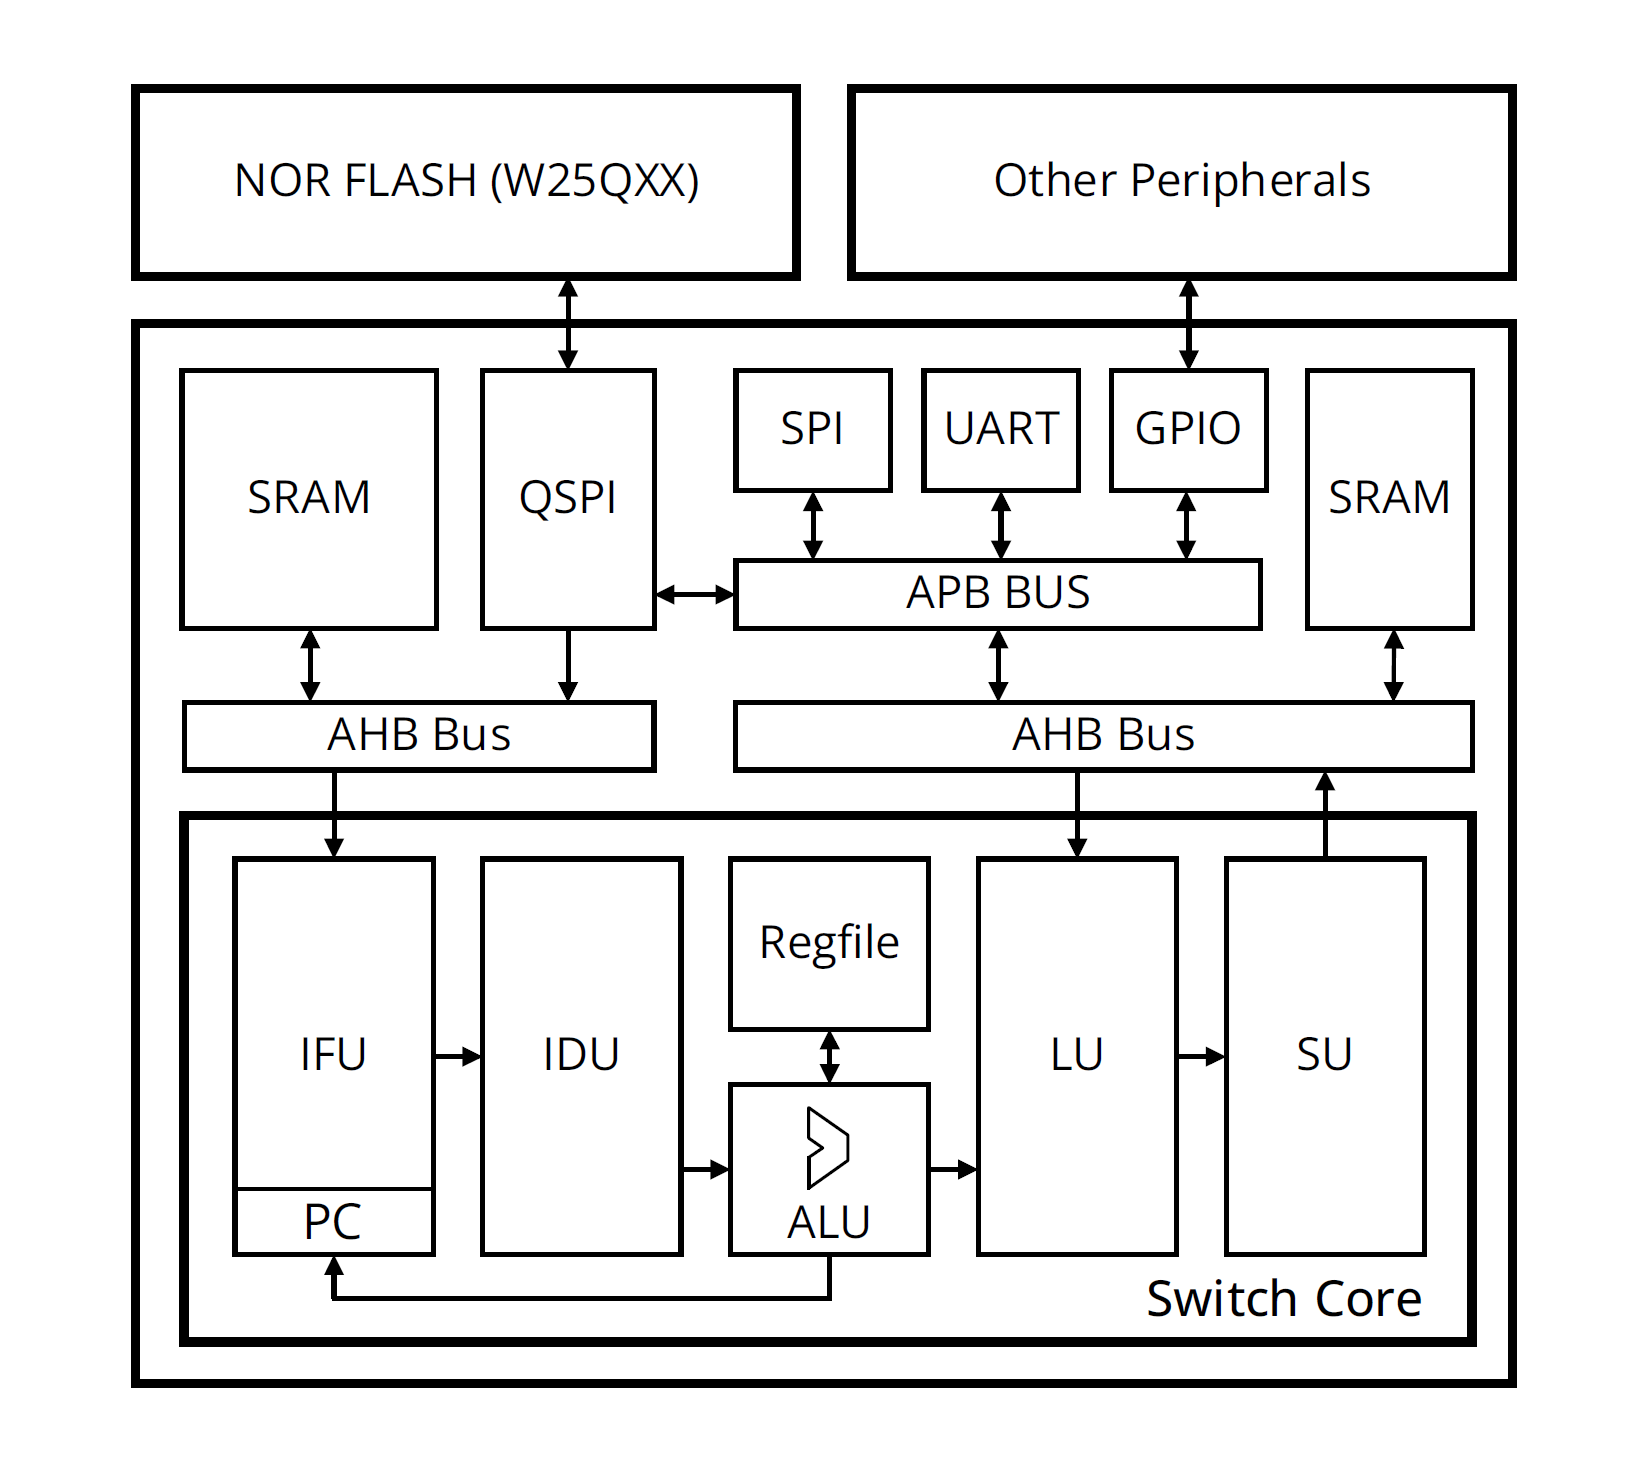
\includegraphics[width=\linewidth]{fig1.png} 
    \caption{System-Level Diagram of the RISC-V Based SwitchMCU.}
    \label{fig}
\end{figure}

The project can be broadly divided into two main sections: the core design and the physical design, which is the main focus of this paper. Physical design can be defined as “the process of transforming a circuit description into the physical layout, which describes the position of cells and routes for the interconnections between them.” \cite{b3}

The core team designs, debugs, and verifies the RISC-V core, and will ultimately produce synthesizable RTL code to be passed along to the physical design team, which consists of the two authors. Once the Verilog code is received, it will be synthesized and ultimately taped out into a reproducible, manufactured chip.

As mentioned previously in the abstract, there is currently no standardized RISC-V Application-Specific Integrated Circuit (ASIC) workflow at Rice University. This is compounded by a more generalized problem in open-source physical design flows, which is confusing or poor documentation. This makes it difficult or even impossible for reproduction and restricts access to only those who are very familiar with the subject.

Therefore, the main assignments of this semester for the physical design team are providing fully documented instructions for each step of the physical design process, a GitHub repository (S25\_pd) with all necessary TCL script files and code, and successfully synthesizing the RTL all the way to generating a GDSII layout. By next semester, the design should meet performance, power, and area (PPA) constraints, and also be ready for actual tapeout with minor modifications.



\section{Methods}
However, current work from the previous semesters requires revisions and additions before it is able to be transferred to a manufacturable chip. Therefore, a simple register file (\texttt{regfile.v}) from ELEC 526: High Performance Computer Architecture will be used as a substitute until the core team is able to complete the processor.

This file is then fed through a simplified physical design flow provided by ELEC 527: VLSI Systems Design Framework. These steps begin with a functional simulation in Questa. The design and testbench files, written in Verilog are compiled, simulated, and run in the GUI. The waveforms are then analyzed to check for any potential issues. Next, the output(s) are passed along to Synopsys Design Compiler for synthesis, which is the process of converting RTL into a gate-level netlist using standard cells. The design is optimized for performance, power and area (PPA) constraints. The synthesized Verilog output is then once again examined in Questa. The final component is place and route in Innovus. The software reads the netlist, places the standard cells within the chip layout, routes the interconnections between the cells, and generates both a physical design report and a GDSII layout. Since the AND structure files provided for this assignment have already been validated and refined, many intermediary steps between synthesis and place and route have been excluded. 

\subsection*{Physical Design Flow}

The full edited physical design flow for this project can be seen below in Fig.2:

\begin{enumerate}
    \item \textbf{Synthesis} - Originally, synthesis was attempted using Library Compiler with an input of \texttt{.lib} and an output of \texttt{.db}. A TCL script was created to convert all \texttt{.lib} files to \texttt{.db} files automatically due to the high volume of these found in the SkyWater 130nm PDK. The \texttt{.db} file is forwarded to Design Compiler, which outputs a \texttt{.vg} file. (For the final design, the file will be also verified in Questa Post DC after initial synthesis with the help of the core design team.) But because of the complexities present in the modified Skywater PDK used in the project, this approach proved problematic in later stages. More about this is discussed in the later section. However, these steps are still applicable for standard synthesis using a general PDK.
    
    \item \textbf{Floorplanning in Innovus} - The file is sent to Innovus for floorplanning, which “is the process of creating core area, specifying core to I/O boundary spacing, standard cell rows, placing I/O pins, placing macros using macro guidelines, and adding placement blockages and halo.” \cite{b4}
    
    \item \textbf{Place and Route (P\&R)} - Like floorplanning, place-and-route is achieved in Innovus. This is the physical implementation stage where logic cells are arranged and interconnected on a chip, and then streamlined. Since there were numerous \texttt{.lef} files in Skywater with duplicates, a TCL script was written to do this explicitly while avoiding the repetitive cases.

    \item \textbf{Clock Tree Synthesis (CTS)} - The final step in Innovus is CTS, which “aims to minimize the routing resources used by the clock signal. Additionally, it minimizes the area occupied by the clock repeaters while meeting an acceptable clock skew, a reasonable clock latency, and clock transition time.” \cite{b5}
    
    \item \textbf{Parasitic Extraction (PEX)} - The \texttt{.gds} file is then given to StarRC for parasitic extraction, also known as Resistance-Capacitance (RC) extraction. This process involves determining both the resistance and capacitance values of interconnections and devices in a circuit layout to more accurately model signal delays and timing behavior.

    \item \textbf{Static Timing Analysis (STA)} - The extracted file(s) are scrutinized in PrimeTime, during which the static timing analysis “provides full chip timing with signal integrity, advanced node accuracy, and ECO guidance.” \cite{b6} As the name suggests, this stage is crucial for ensuring correct and reliable timing in the design.
    
    \item \textbf{Design Verification} -  The last part of the physical design flow is design verification using Calibre, which can be dissected into two parts: Design Rule Checks (DRC) and Layout Versus Schematic (LVS). DRC is used to verify that the physical layout of the chip adheres to the restrictions and requirements set by the manufacturer. Meanwhile, the purpose of the LVS is to verify that the layout of the chip is representative of the netlist.

\end{enumerate}

After all seven phases have been successfully completed, the design can be sent to the manufacturer for tapeout. Actual tapeout can span across a period of several months. 

\begin{figure}[htbp]
    \centering
    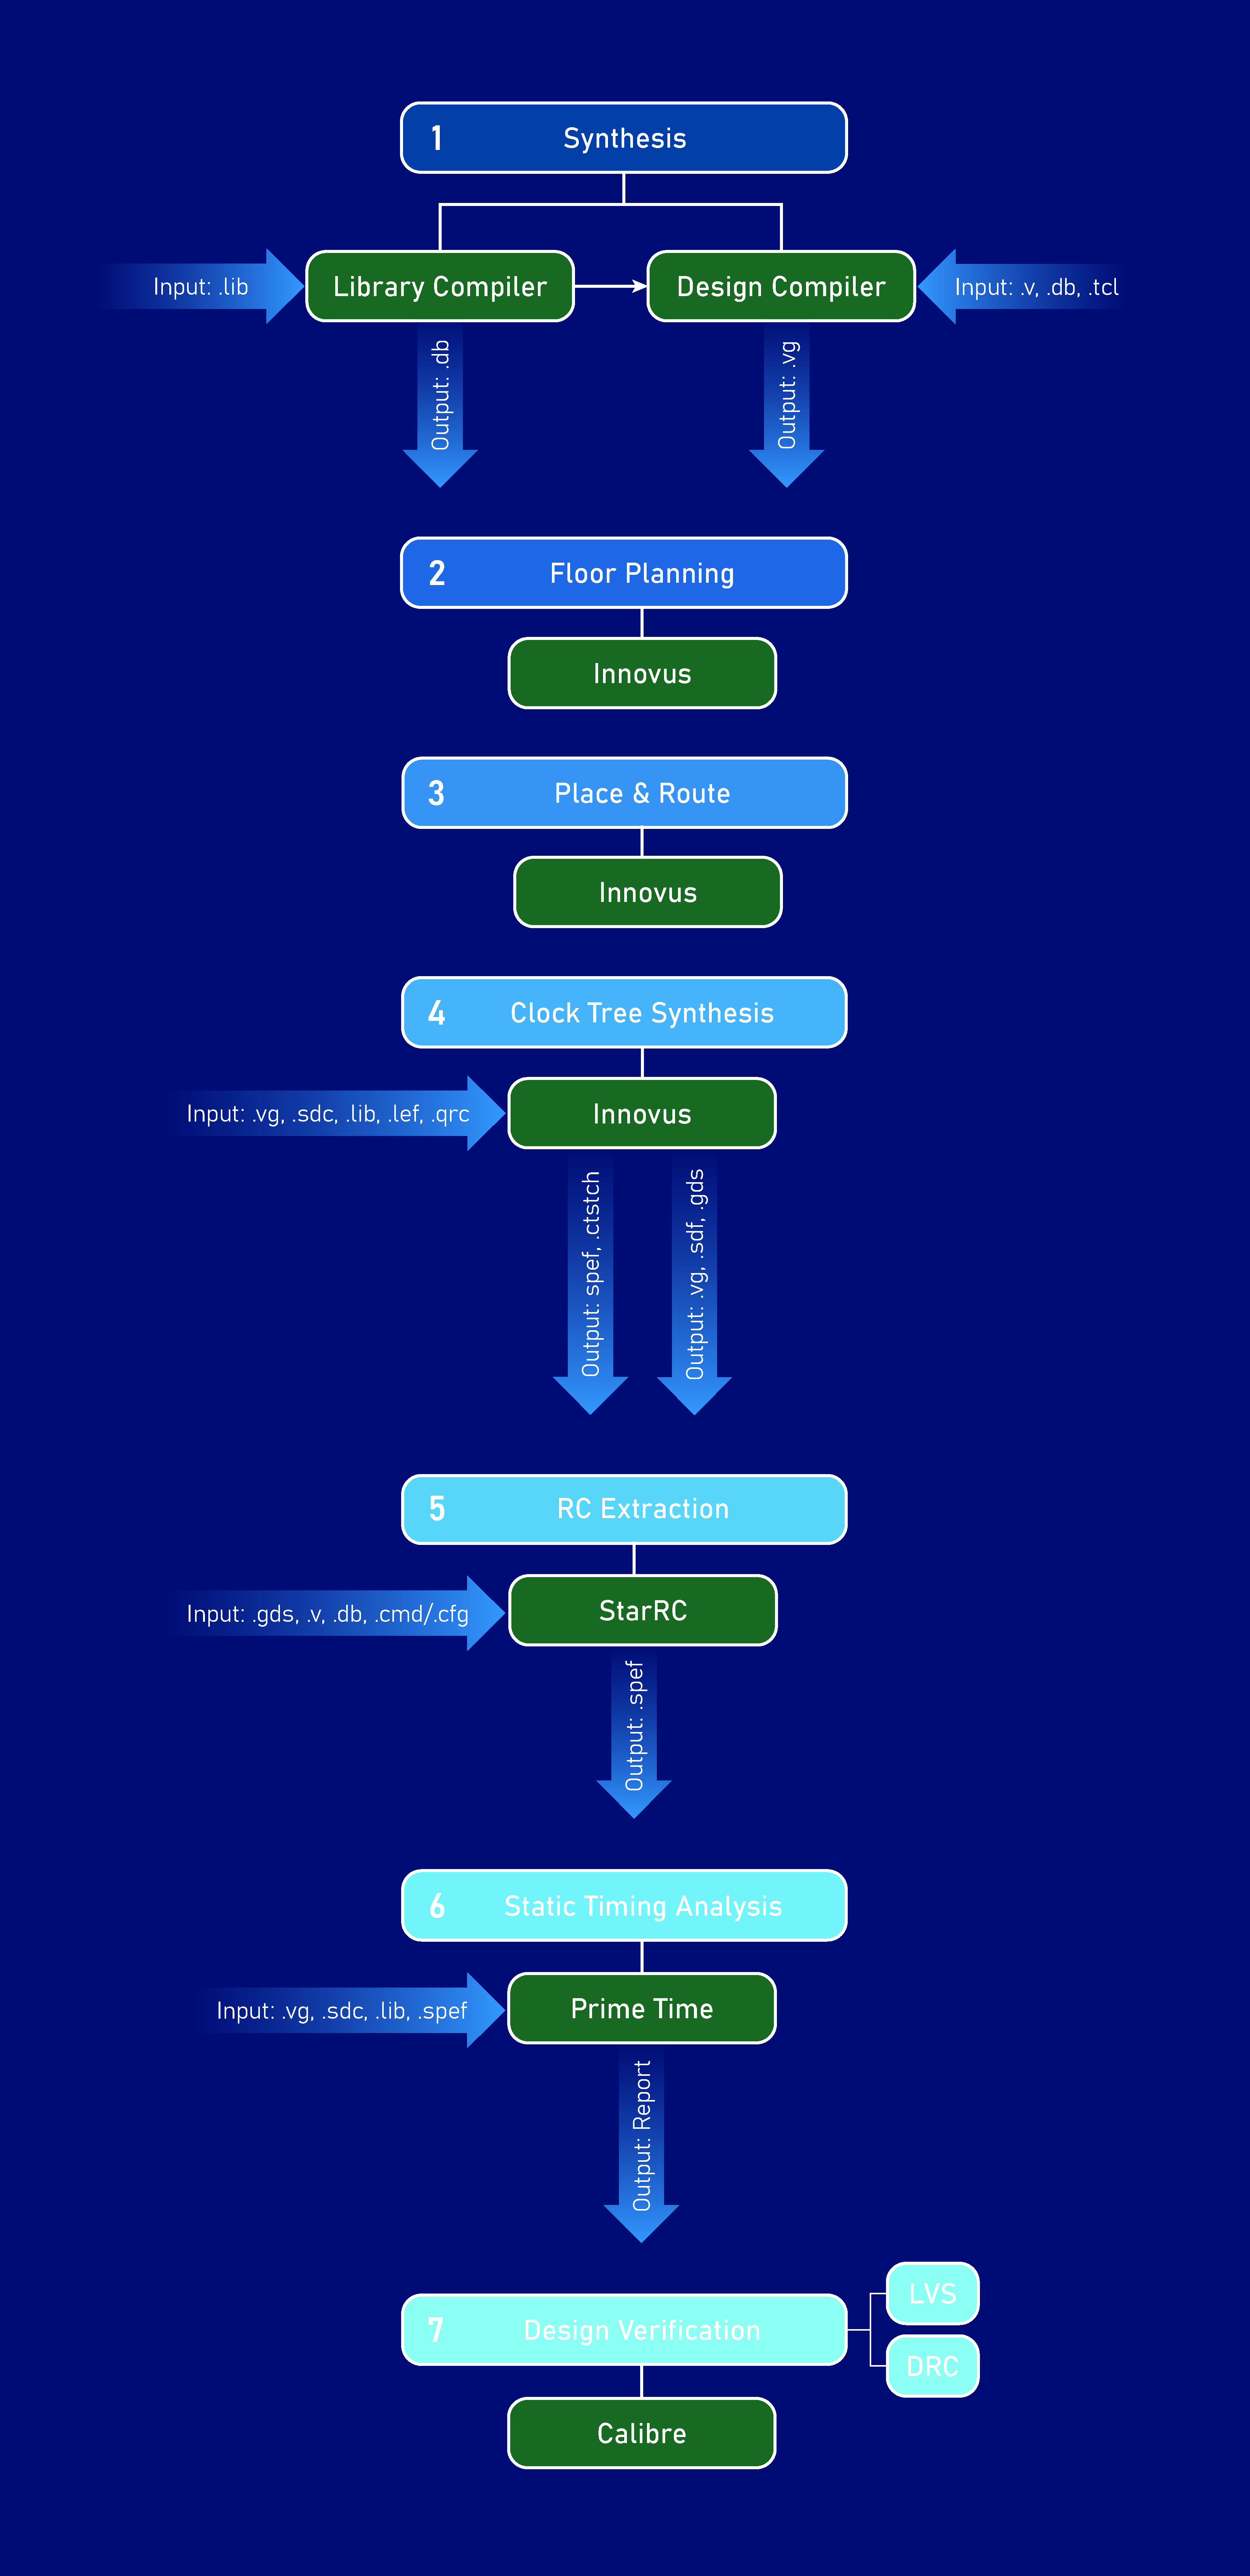
\includegraphics[width=\linewidth]{fig2.jpg} 
    \caption{Physical design flow.}
    \label{fig}
\end{figure}

\section{Results}

Current progress at the time of this report is around 60\%. For the next semester, there remains: RC extraction, static timing analysis,  physical verification and post synthesis simulation for the regfile. After successfully completing the physical design flow with this stand-in file, the core design (or a similar alternative if it has not yet been completed) will be adapted to the framework. Eventually, it will be taped out into a fabricated chip. Since the core team has not finished all the RTL code, the following results are based only on the register file block. 


The total number of cells used, along with the area, timing, and power results based on the SkyWater PDK, are shown in Fig. 3:

\begin{figure}[htbp]
    \centering
    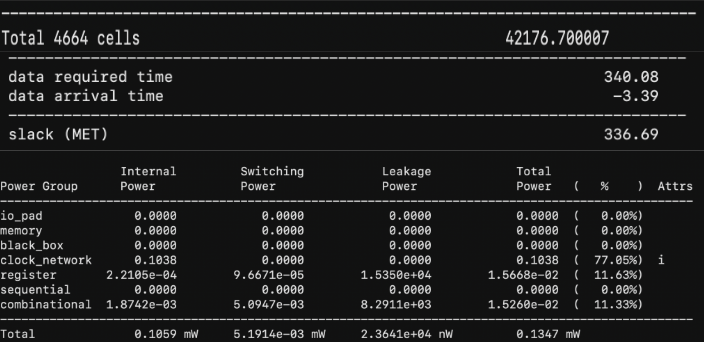
\includegraphics[width=\linewidth]{fig3.png} 
    \caption{Area, timing, and power after synthesis.}
    \label{fig3}
\end{figure}

Fig. 4  and Fig. 5 illustrate DRC verification results and final layout after detail routing

\begin{figure}[htbp]
    \centering
    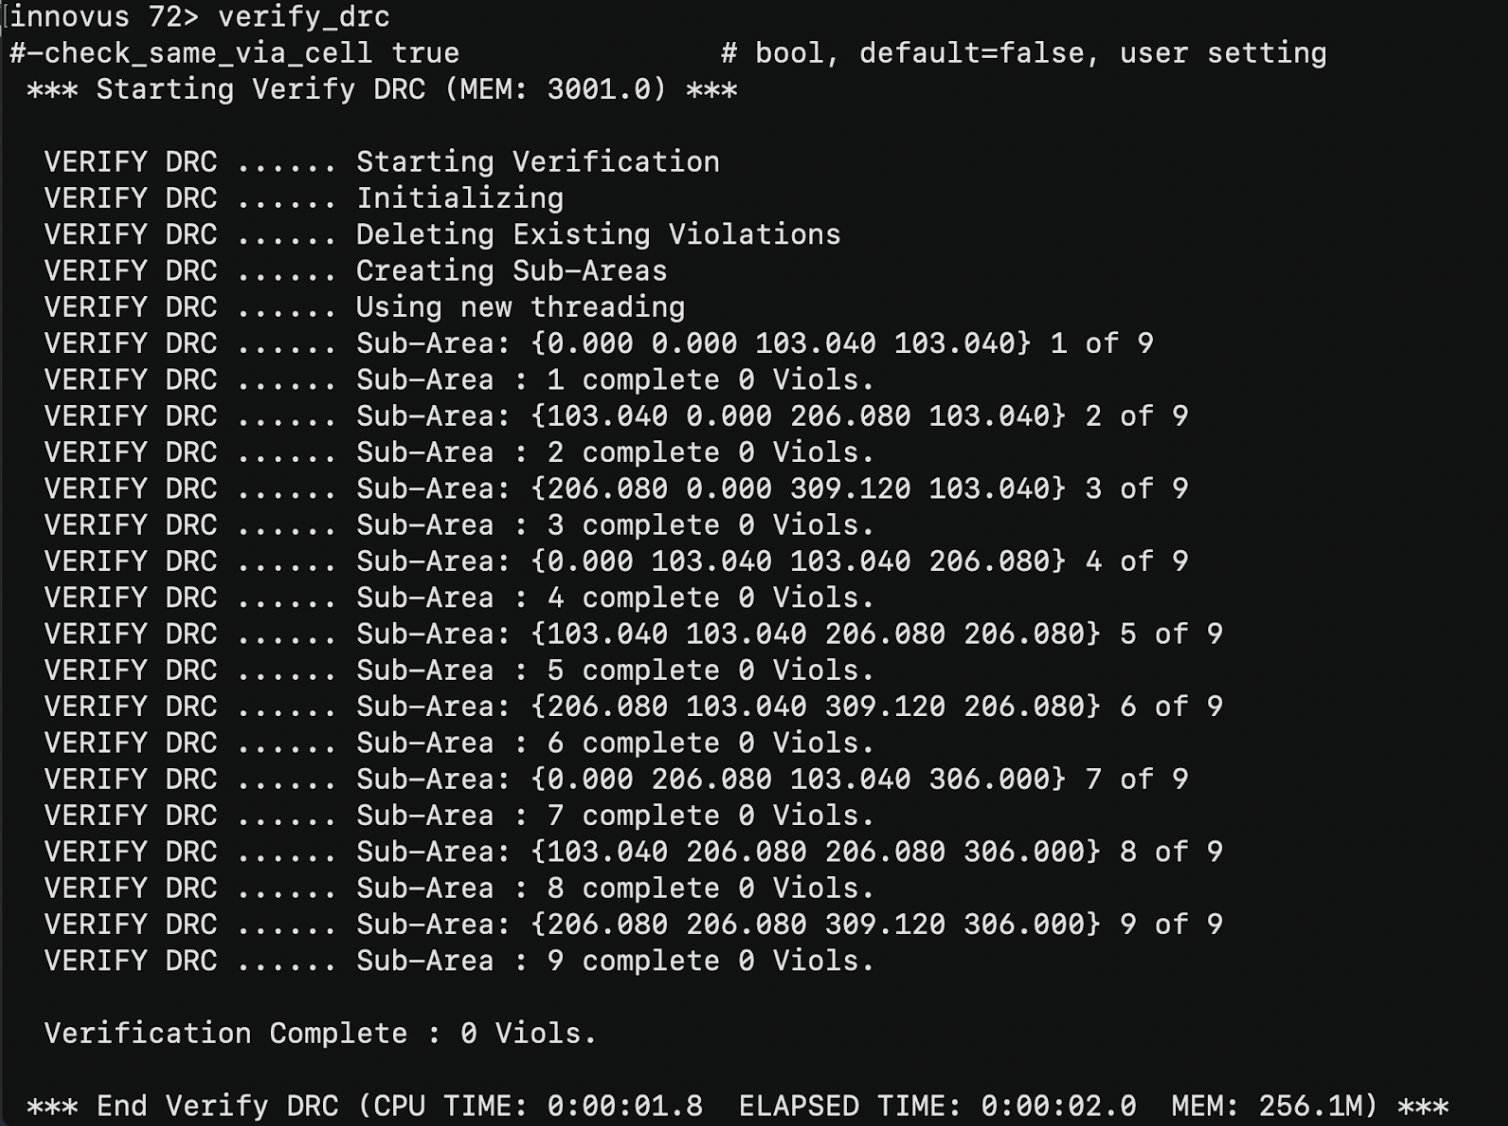
\includegraphics[width=\linewidth]{fig4.png} 
    \caption{DRC verification results.}
    \label{fig4}
\end{figure}

\begin{figure}[htbp]
    \centering
    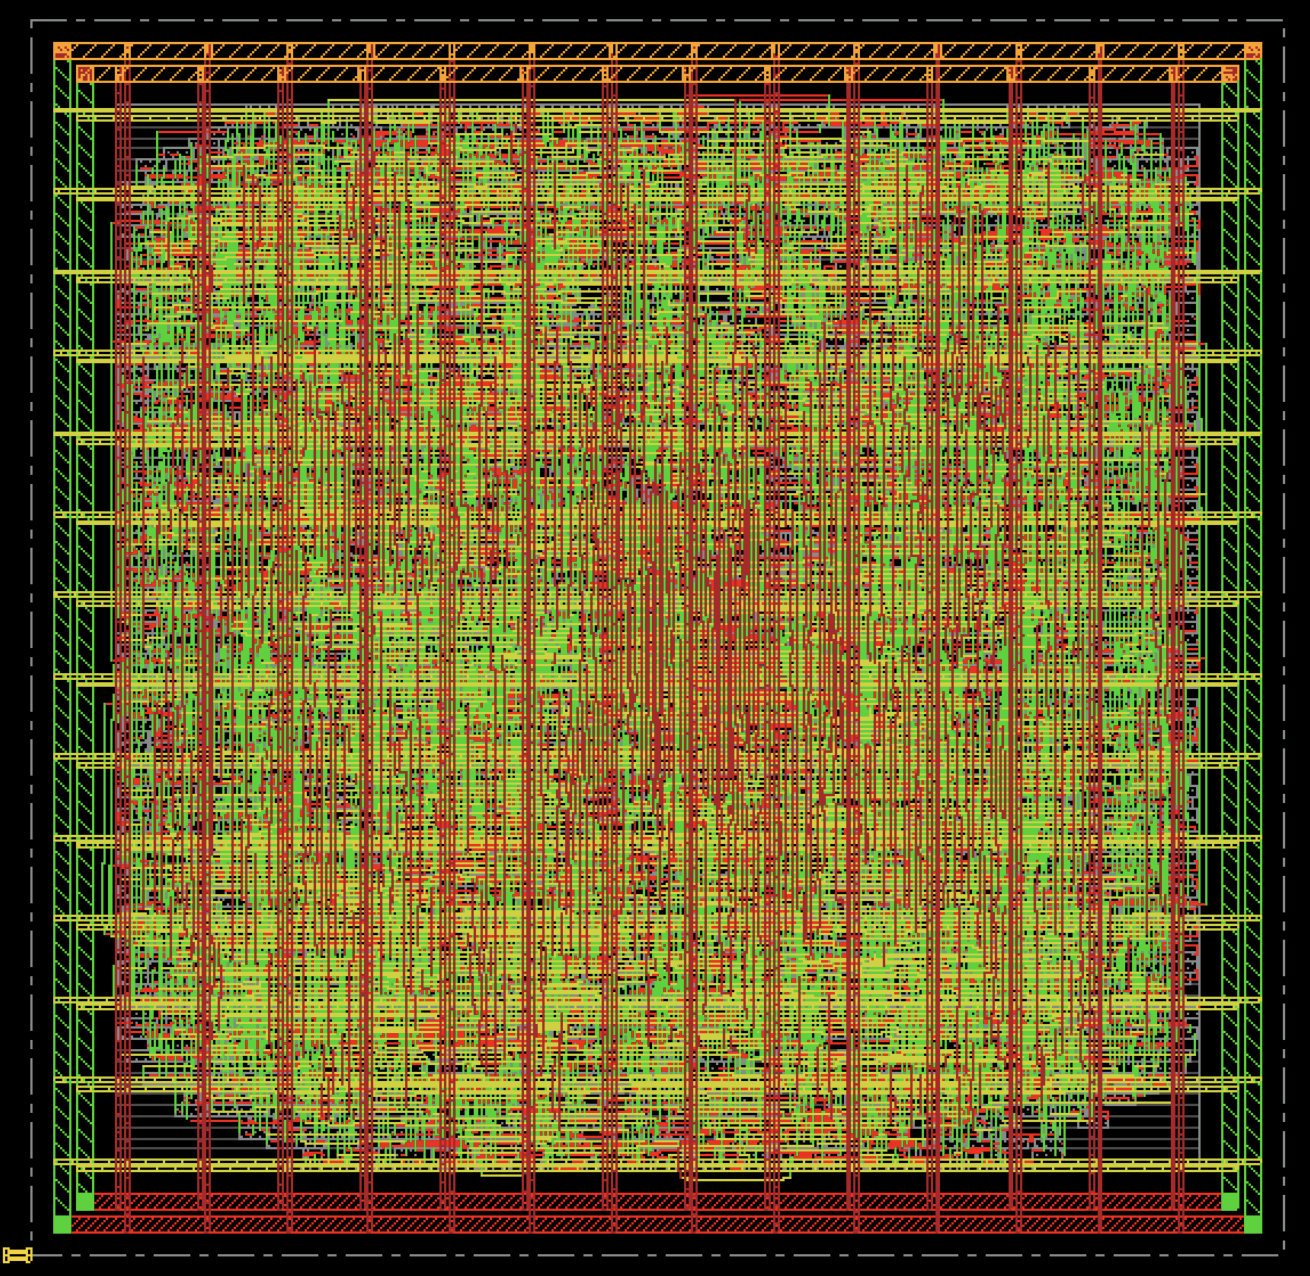
\includegraphics[width=\linewidth]{fig5.png} 
    \caption{Layout results from the place-and-route stage.}
    \label{fig5}
\end{figure}

\section{Discussion}
One major setback was multiple issues in the initial attempts at routing. Originally, duplicate information from the Skywater 130nm PDK was merged, creating issues that needed correcting before the physical design flow could continue. The three main barriers found were routing issues, failure to the build timing graph, and GDS file incompatibility.

Therefore, it was necessary to take a step back and repeat synthesis using a different approach. By modifying the python code provided by Timothy Edwards on Github, the .lef were successfully merged.\cite{b7}

This step will require the Python library “natsort” if it has not already been installed. Next, place and route also required a new strategy as timing should be considered during optimized placement. First the multi mode multi corners (mmmc) were created for optimized placement and the qrc file was downloaded from Github. Normally the foundry would be contacted for the mmmc details, however it is unnecessary at this moment, and only two corners were created. After this step has been completed, the design is optimized and then placed. Before routing, it is recommended to verify the connectivity and periodically conduct DRC checks to spot any underlying issues. Because the file was only routed globally, there were plenty of  errors and connectivity issues present. These should be rectified after detailed routing and can be ignored at this stage. The subsequent procedure is to synthesize the clock tree, which is a standard part of any physical design flow. For this reason, it was attempted with the regfile.v even though it only has one clock. There were two errors regarding connectivity, but they were corrected using the command “nanoRoute”. And finally, the detail route is completed.

Comparatively, the file currently used in the design flow is a rudimentary, clean register that is much more straightforward than the completed core design. Thus, adapting the actual SwitchMCU core to the development process will likely introduce even more significant drawbacks and difficulties.


\section*{Acknowledgment}

We would like to express our sincerest gratitude to Professor Yu Kee Ooi for this interesting and valuable semester thus far, as well as both Joe Cavallaro and Peter Varman for their resources used by the physical design team. From Joe Cavallaro, the physical design flow framework and files, and from Peter Varman, the regfile.v used in each stage of the methodology. 

\begin{thebibliography}{00}
\bibitem{b1} Synopsys, “What is RISC-V? – How does it work?,” 
\emph{Synopsys}, \url{https://www.synopsys.com/glossary/what-is-risc-v.html} 
(accessed Mar. 13, 2025).
\bibitem{b2} Rice-MECE-Capstone-Projects, “SWITCHMCU: Switch MCU Repository,” 
\emph{GitHub}, \url{https://github.com/Rice-MECE-Capstone-Projects/SwitchMCU} 
(accessed Mar. 13, 2025).

\bibitem{b3} K. Sharma, “What is Physical Design,” 
\emph{VLSI - Physical Design For Freshers}, 
\url{https://www.physicaldesign4u.com/2019/12/what-is-physical-design.html} 
(accessed Mar. 13, 2025).

\bibitem{b4} VLSI Talks, “Floorplanning in Physical Design,” 
\emph{VLSI TALKS}, 
\url{https://vlsitalks.com/physical-design/floorplan/} 
(accessed Mar. 13, 2025).

\bibitem{b5} AnySilicon, “Ultimate Guide: Clock Tree Synthesis,” 
\emph{AnySilicon}, 
\url{https://anysilicon.com/clock-tree-synthesis/} 
(accessed Mar. 13, 2025).

\bibitem{b6} Synopsys, “PrimeTime: Static Timing Analysis,” 
\emph{Synopsys}, 
\url{https://www.synopsys.com/implementation-and-signoff/signoff/primetime.html} 
(accessed Mar. 13, 2025).

\bibitem{b7} R. T. Edwards, “create lef library” 
\emph{GitHub}, 
\url{https://github.com/RTimothyEdwards/open_pdks/blob/master/common/create_lef_library.py} 
(accessed Mar. 13, 2025).

\end{thebibliography}


\end{document}
